\chapter{Replace with Title}
\label{ch:chapter1}

Please remove this instructional text and replace it with your work.

Text in the body of your work may be single, double, or one-and-a-half
spaced. This template uses double spacing (set by \verb|\doublespacing| in
\texttt{psu-dissertation.cls}).

Chapter headings use \verb|\chapter|. Subheadings begin with \verb|\section|
and go in numerical order through \verb|\subsection| and
\verb|\subsubsection|.

\section{Replace with subheading}

\subsection{Replace with subheading}

\subsubsection{Replace with subheading}

\section{Page Breaks}

Each chapter starts on a new page automatically, so no manual page or
section breaks are needed. In the Word template, these breaks are shown with
the Show/Hide~\P{} button (\autoref{fig:show-hide}).

\begin{figure}[htbp]
  \centering
  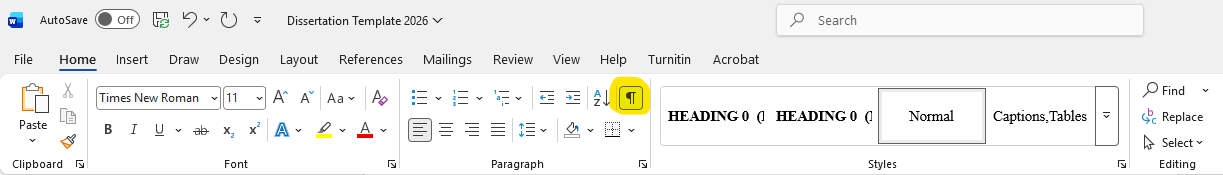
\includegraphics[width=0.5\textwidth]{show-hide}
  \caption{Show/Hide \P}
  \label{fig:show-hide}
\end{figure}
